Ahora procedemos a comprobar la hermiticidad de la caja oscura en el interior de la cual se desarrollará el experimento. Para ello preparamos 3 muestras diferentes de fibras no clad de $200~\mm$ de longitud y realizamos una medición de cada una de estas para cuatro intensidades diferenets de alimentación de la LED. Seguidamenet repetimos el mismo experimento incorporando sobre el prototipo una manta oscura especial para asugurar la total hermiticidad del sistema a los fotones.

En la figura \ref{plotmanta} podemos observar las señales promediadas de ambos experimentos con su desviación estandar, la cual se muestra inapreciable a esta escala.

\begin{figure}[H]
\centering
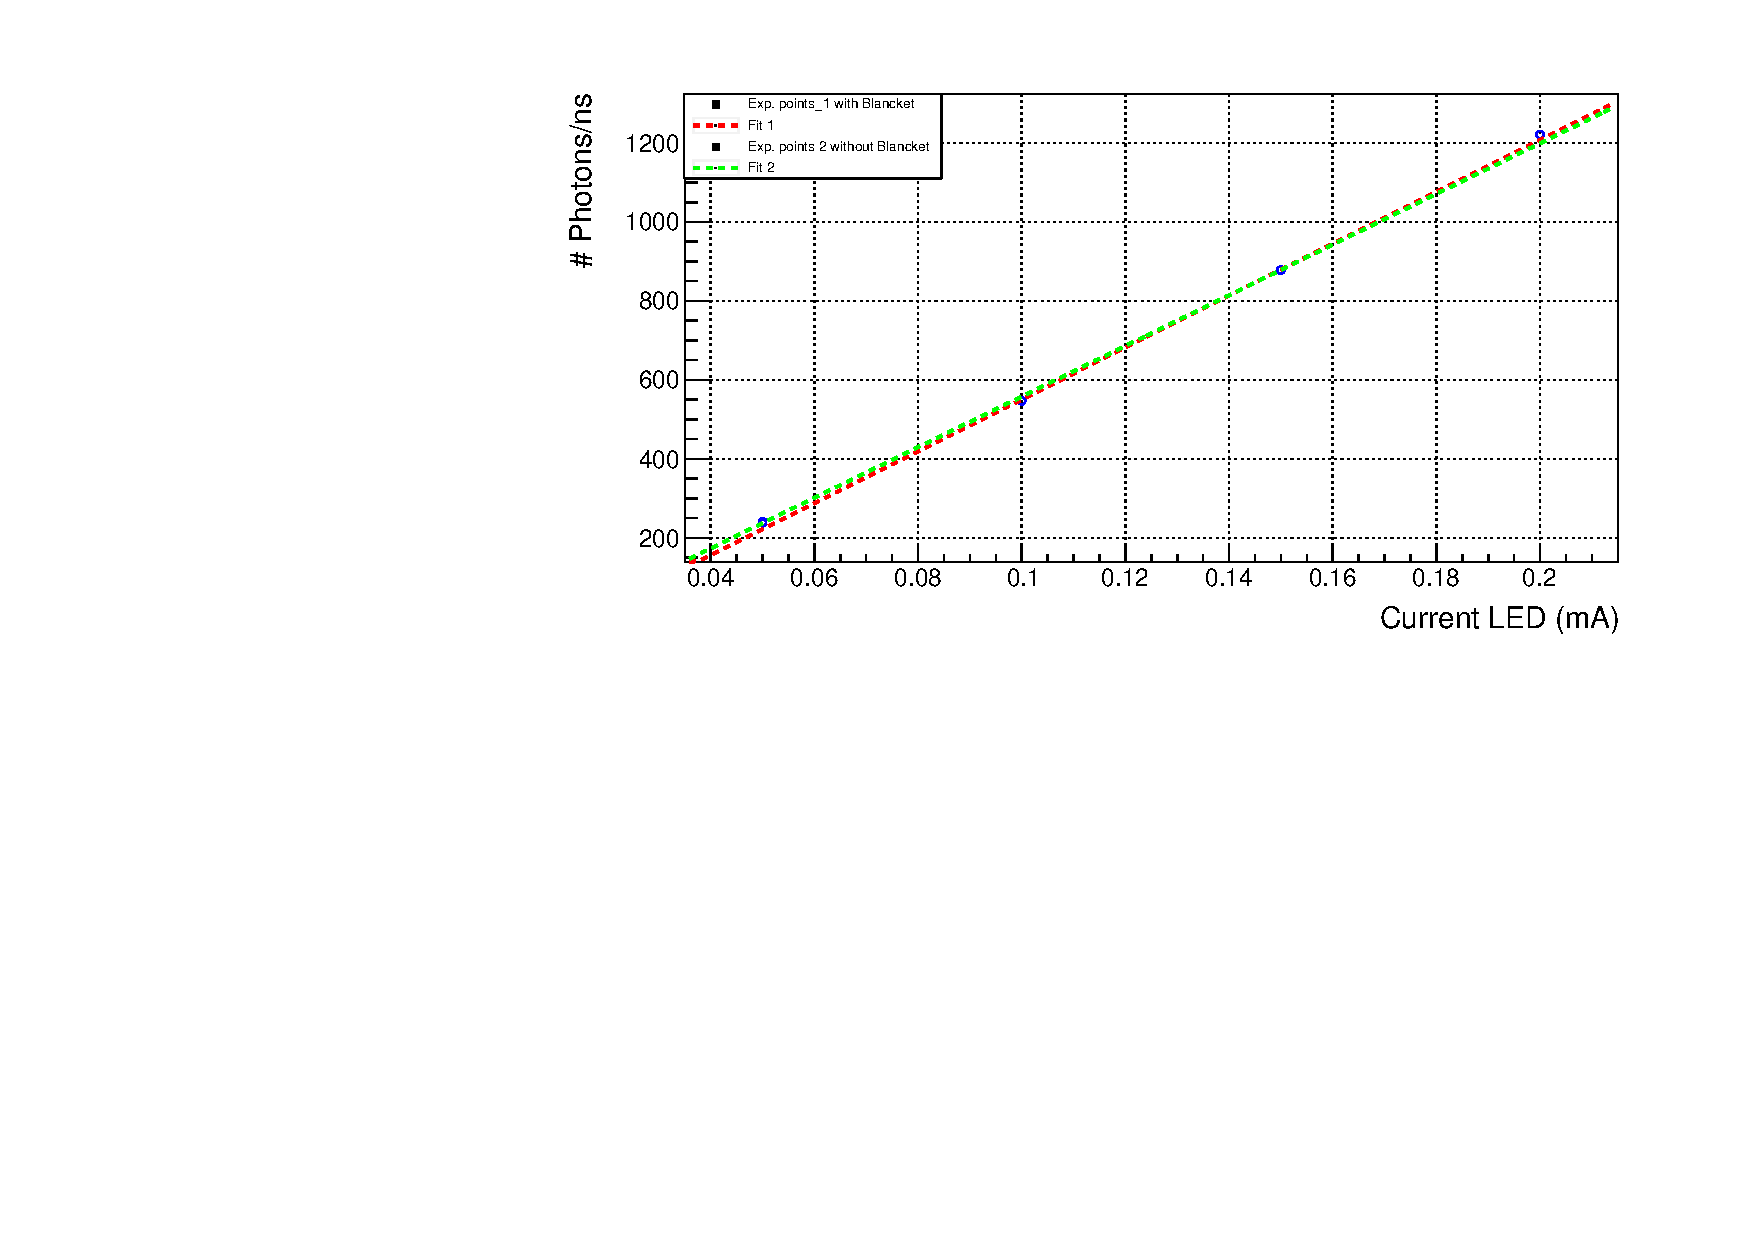
\includegraphics[scale=0.7]{Figuras/cases.pdf}
\caption{Señales medidas con y sin manta para fibras no clad de $200~\mm$\label{plotmanta}}
\end{figure}

Podemos observar que la señal es aproximadamente la misma. Finalmente representamos en la figura \ref{diferencia} la resta entre ambas señales.

\begin{figure}[H]
\centering
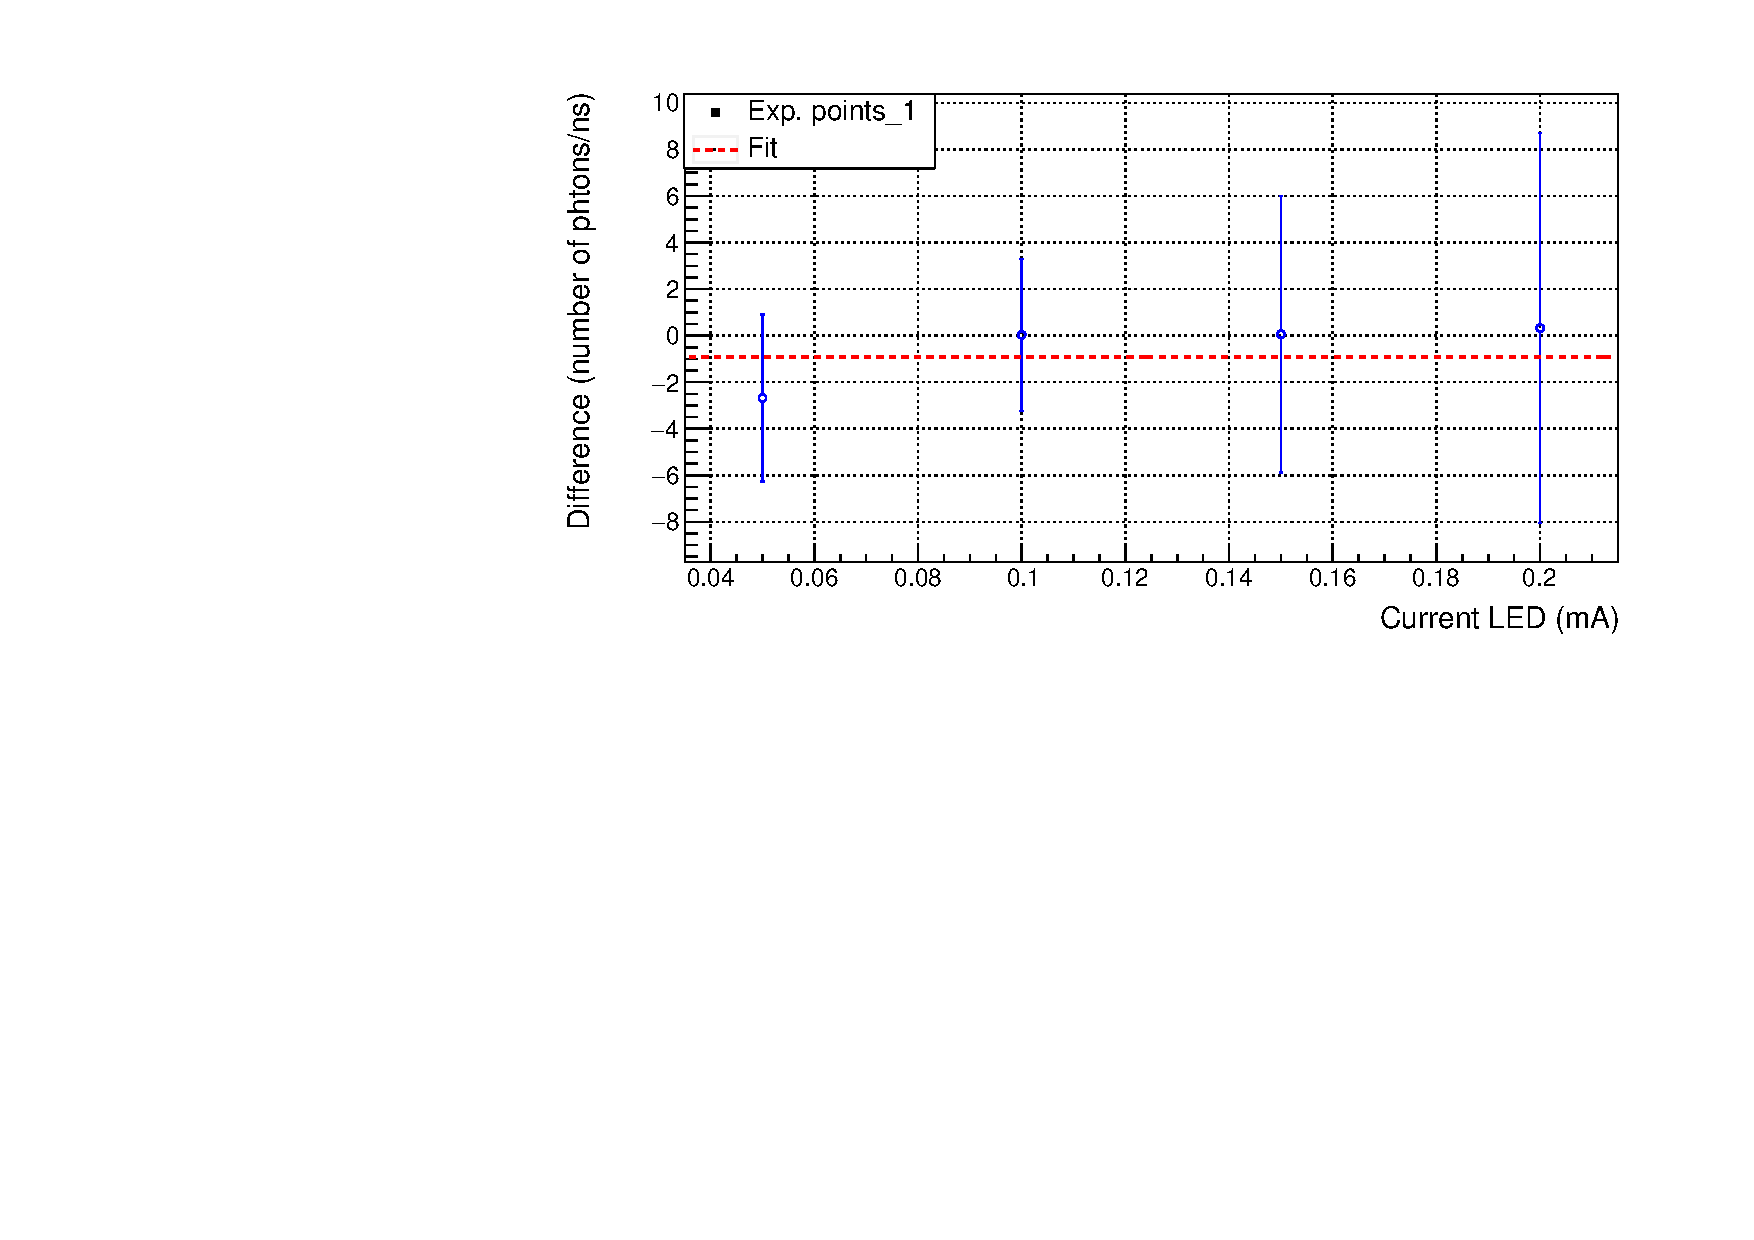
\includegraphics[scale=0.7]{Figuras/difference.pdf}
\caption{Diferencia entre las señales medidas con y sin manta para fibras no clad de $200~\mm$\label{diferencia}}
\end{figure}

Podemos observar que la diferencia es prácticamente nula. Con la propagación de incertidumbres vemos que las mínimas diferencias entres estas señales pueden explicarse perfectamente con la estadística. La razon de tener incertidumbres grandes es que este resultado se ha obtenido con la resta dos valores muy cercanos y muy grandes. Debido a ello tendremos errores superiores al valor numérico.



